\lesson{original Lecture 3 -- 5}{Data Reduction}
\subsection{Sufficiency}
\begin{definition}[statistic]
    A statistic $T:\mathcal{X}\to \mathcal{T}$ is a function of data
\end{definition}

\begin{example}[sample mean is a statistic.]
    \begin{gather}
        T(\boldsymbol{X})=\frac{1}{n}\sum_{i=1}^n{X_i}\triangleq\bar{X}_n
    \end{gather}
\end{example}

\begin{definition}[sufficient statistic]
    A statistic is sufficient for a model $\mathcal{P}=\{p_\theta:\theta\in\Omega\}$
    if for all $t$, the conditional distribution $X|T(X)=t$ does not depend on $\theta$, i.e. 
    \begin{gather}
        X|T(X)=t\vperp \theta.
    \end{gather}
\end{definition}

\begin{note}
    The $X$ above should be all samples and cannot be partial.
\end{note}

\begin{example}
    Let $X_1,\cdots,X_n\overset{iid}{\sim}\text{Bernoulli}(\theta)$.
    Is $\sum_{i=1}^n{X_i}$ ($\sim \text{Bin}(n,\theta)$) sufficient?
    \begin{align}
        P_\theta(\boldsymbol{X}=\boldsymbol{x}|T(\boldsymbol{X})=t)
        =&\frac{P_\theta(\boldsymbol{X}=\boldsymbol{x},T(\boldsymbol{X})=t)}{T(\boldsymbol{X}=t)}\\
        =&\frac{\mathbb{I}(\sum_{i=1}^n{X_i}=t)\theta^t(1-\theta)^{n-t}}{\binom{n}{t}\theta^t(1-\theta)^{n-t}}\\
        =&\frac{\mathbb{I}(\sum_{i=1}^n{X_i}=t)}{\binom{n}{t}}\\
        =&\frac{1}{\binom{n}{t}}
    \end{align}
\end{example}

\begin{example}
    Let $X_1,\cdots,X_n\overset{iid}{\sim}\text{U}(0,\theta)$. 
    Show that $T(\boldsymbol{X})=\max_{1\leq\ i\leq n}X_i\triangleq X_{(n)}$ is sufficient.
    \begin{align}
        F_T(t)=&P(T\leq t)=P(\max_{1\leq\ i\leq n}X_i\leq t)\\
        =&P(X_1\leq t,\cdots,X_n\leq t)=[P(X_1\leq t)]^n=\left(\frac{t}{\theta}\right)^n\\
        \Rightarrow
        f_T(t)=&\frac{nt^{n-1}}{\theta^n}~\text{and}~
        P(\boldsymbol{X}|T))=\cdots\vperp\theta
    \end{align}
\end{example}

\begin{example}
    The order statistics $T(\boldsymbol{X})=(X_{(1)},\cdots,X_{(n)})$ 
    from a random sample of $X_i\overset{iid}{\sim}f$ are sufficient.
    Given $T(\boldsymbol{X})$, the possible values of $X$ are $n!$ permutation of $T$:
    \begin{gather}
        P(X_1=X_{(1)},\cdots,X_n=X_{(n)})=\frac{1}{n!}
    \end{gather}
\end{example}


\begin{theorem}
    If $X\sim p_\theta\in\mathcal{P}$ and $T$ is sufficient for $\mathcal{P}$,
    then for any decision procedure $\delta$,
    there is a (possibly randomized) decision procedure of equal risk that depends on $X$ through $T(\boldsymbol{X})$ only.
\end{theorem}

\begin{note}
    Suppose we are given an independent source of randomness, 
    say $U\vperp\theta$, we can generate a new dataset $\boldsymbol{X}'$ 
    from the conditional distribution $P(\boldsymbol{X}|T(\boldsymbol{X}))$ and define a randomized procedure:
    \begin{align}
        \delta^*(\boldsymbol{X},U)\triangleq\delta(f(T(\boldsymbol{X})),U)
        =\delta(\boldsymbol{X}')\overset{d}{=}\delta(\boldsymbol{X})
    \end{align}
\end{note}


\begin{example}
    $X, Y\overset{iid}{\sim}f_\theta$, where $f_\theta(x)=\left\{\begin{array}{ll}
        \theta e^{-\theta x} & x\geq 0 \\
        0 & \text{otherwise}
    \end{array}\right.$.
    Let $U\sim\text{Uniform}(0,1)\vperp(X,Y)$. 
    Define $T=X+Y$, $\tilde{X}=UT$ and $\tilde{Y}=(1-U)T$ ($\Rightarrow\tilde{X}+\tilde{Y}=X+Y$).
    \begin{align}
        P(T\leq t|Y\leq y)
        =& P(X+Y\leq t|Y=y)\\
        =& \mathbb{E}(\mathbb{I}(X+Y\leq t)|Y=y)\\
        =& \int\mathbb{I}(x\leq t-y)dF_X(x)\\
        =& F_X(t-y)
    \end{align}
    We can write $P(T\leq t|Y)=F_X(t-Y)$, a function of r.v. $Y$.
    \begin{align}
        P_T(t)
        =& P(T\leq t) = \mathbb{E}_Y(F_X(t-Y))\\
        =& \int_{0}^t{(1-e^{-\theta(t-y)})\theta e^{-\theta y}}dy\\
        =& 1-e^{-\theta t} - t\theta e^{-\theta t}
    \end{align}
    which gives $f_T(t)=\frac{\partial F_T(t)}{\partial t}=t\theta^2e^{-\theta t}$, $t\geq 0$.

    Note that $(U,T)$ has the joint density
    \begin{align}
        p_\theta(t,u)=&\left\{\begin{array}{ll}
            t\theta^2e^{-\theta t} & t\geq 0,u\in(0,1) \\
            0 & \text{otherwise}
        \end{array}\right.\\
        P_\theta((\Tilde{X},\Tilde{Y})\in B)=&\iint_{B}(tu,(1-u)t)p_\theta(t,u)dudt
    \end{align}
    Hence, $\Tilde{X}$ and $\Tilde{Y}$ have the joint density of
    \begin{gather}
        \frac{p_\theta(x_y,\frac{x}{x+y})}{x+y}=\left\{\begin{array}{ll}
            \theta^2e^{-\theta(x+y)} & x\geq 0,y\geq 0 \\
            0 & \text{otherwise}
        \end{array}\right.
    \end{gather}
    which is the same joint density as $(X,Y)$.
\end{example}

\begin{theorem}
    \textbf{Neymann-Fisher Factorization Criterion}\\
    Suppose each $p_\theta\in\mathcal{P}$ has density $p(x;\theta)$ 
    with respect to a common $\sigma$-finite measure $\mu$, 
    i.e. $\frac{dP_\theta}{d\mu}=p(x;\theta)$. 
    Then, $T(\boldsymbol{X})$ is sufficient if and only if 
    \begin{gather}
        p(\boldsymbol{x};\theta)=g_\theta(T(\boldsymbol{x}))h(\boldsymbol{x})
    \end{gather}
    for some functions $g_\theta$ and $h$ where $h(\boldsymbol{x})$ is free of $\theta$.
\end{theorem}
\begin{proof}
    Refer to Casella and Berger, 2001.
\end{proof}

\begin{example}
    Let $X_1,\cdots,X_n\overset{iid}{\sim}\mathcal{N}(\mu,\sigma^2),~\theta=(\mu,\sigma^2)$. 
    The joint distribution of $(X_1,\cdots,X_n)$ is 
    {\scriptsize \begin{align}
        &p(\boldsymbol{x};\theta)= \prod_{i=1}^n\frac{1}{\sqrt{2\pi\sigma^2}}
        \exp\left\{ -\frac{(x_i-\mu)^2}{2\sigma^2} \right\}\\
        &= \left(\frac{1}{\sqrt{2\pi\sigma^2}}\right)^n\exp\left\{ 
        \frac{1}{2\sigma^2}\left( -\sum_{i=1}^n{x_i^2}+2\mu\sum_{i=1}^n{x_i}-n\mu^2 \right) 
        \right\}\cdot\prod_{i=1}^n\mathbb{I}(-\infty<x_i<\infty)
    \end{align}}
    We have $T(\boldsymbol{X})=(\sum_{i=1}^nX_i^2,\sum_{i=1}^n{X_i})$.
    By NFFC, we claim that $T$ is sufficient for $\theta$ (or $p_\theta$).
\end{example}


\subsection{Exponential Families}
The model $\mathcal{P}=\{p_\theta:\theta\in\Omega\}$ forms an s-dimensional exponential family 
if each $p_\theta$ has the density of the form:
{\Large
\begin{gather}
    p(x;\theta)=\exp\left\{ \sum_{i=1}^s 
    \overbrace{\eta_i(\theta)}^\text{\tiny \color{red} nat. param.} 
    \underbrace{T_i(x)}_\text{\tiny \color{red} suff. stat.}
    -\overbrace{B(\theta)}^\text{\tiny \color{red} standardizer} \right\}
    \underbrace{h(x)}_\text{\tiny \color{red} base measure}
\end{gather}}
\begin{gather}
    B(\theta)=\log{
    \int\exp\left\{ \sum_{i=1}^s\eta_i(\theta)T_i(x) \right\}h(x)d\mu(x)
    }\in\mathbb{R}
\end{gather}

\begin{definition}[Exponential family in canonical form]
    An exponential family is in \textbf{\uline{canonical form}} when density has the form:
    \begin{gather}
        p(x;\boldsymbol{\eta})=\exp\left\{ \sum_{i=1}^s\eta_iT_i(x)-A(\boldsymbol{\eta}) \right\}h(x)
    \end{gather}
\end{definition}

\begin{definition}[Natural parameter space]
    The set of all valid natural parameters $\Omega$ is called the natural parameter space for each $\eta\in\Omega$,
    There exists a normalizing constant $A(\boldsymbol{\eta})$ such that $\int{p(x;\boldsymbol{\eta})}dx=1$.
    Equivalently,
    \begin{gather}
        \Omega=\left\{ \eta:0\leq\int\exp\left\{\sum_{i=1}^s\eta_iT_i(X)\right\}h(x)d\mu(x) < \infty \right\}
    \end{gather}
    For any canonical exponential family, $\mathcal{P}=\{f_\eta:\eta\in\mathcal{H}\}$,
    we have $\mathcal{H}\subseteq\Omega$, $\Omega$ is convex.\footnote{refer to TSH, $\S$ 2.7.1}
\end{definition}

\begin{definition}[Unidentifiable]
    If $\mathcal{P}=\{p_\theta:\theta\in\Omega\}$, then $\theta$ is \textbf{\uline{unidentifiable}}
    if for two parameters $\theta_1\neq\theta_2$, $f_{\theta_1}=f_{\theta_2}$.
\end{definition}

\begin{note}
    Two cases when the superficial dimension of a 2-dimensional exponential family $\mathcal{P}$ can be reduced:
    \begin{enumerate}[{(1)}]
        \item $X\sim\text{Exp}(\eta_1,\eta_2)$ with density
        \begin{gather}
            p(x;\eta_1,\eta_2)=\exp\{-\eta_1x-\eta_2x+\log(\eta_1+\eta_2))\}\mathbb{I}(x\geq 0),\label{eq:reducible}
        \end{gather}
        where $T_1(X)=T_2(X)=X$ are linearly dependent. 
        That is the $T_i(X)$'s satisfy an affine equality. 
        Constraint for all $x\in\mathcal{X}$ which will result in unidentifiability, i.e.
        \begin{gather}
            p(x;\eta_1+c,\eta_2-c)=p(x;\eta_1,\eta_2)~\forall{c}<\eta_2
        \end{gather}
        We can actually combine $(\eta_1,\eta_2)$ into $\eta_1+\eta_2$ and rewrite Equation (\ref{eq:reducible}) as 
        \begin{gather}
            p(x;\eta_1,\eta_2)=\exp\{-\underbrace{(\eta_1+\eta_2)}_{\color{red}\eta}x
            +\log\underbrace{(\eta_1+\eta_2)}_{\color{red} \eta}\}\mathbb{I}(x\geq 0)
        \end{gather}
        \item The $\eta_i$'s satisfy an affine equality constraint, for all $\eta\in\mathcal{H}$,
        $p(x;\boldsymbol{\eta})\propto\exp\{\eta_1x+\eta_2x^2\}$ for all $(\eta_1,\eta_2)$ 
        satisfying $\eta_1+\eta_2=1$. 
        Then we can write 
        \begin{gather}
            p(x;\boldsymbol{\eta})\propto\exp\{\eta_1x+\eta_2x^2\}=\exp\{\eta_1(x-x^2)+x^2\}.
        \end{gather}
    \end{enumerate}
\end{note}

\begin{definition}[Minimal]
    A canonical exponential family $\mathcal{P}=\{p_\eta:\eta\in\mathcal{H}\}$ is \textbf{\uline{minimal}} if
    \begin{enumerate}[{(1)}]
        \item No affine $T_i$'s: 
        $\sum_{i=1}^s\lambda_iT_i(x)=\lambda_0~\forall{x}\in\mathcal{X}\Rightarrow\lambda_i=0~\forall{i}\in\{1,\cdots,s\}$
        \item No affine $\eta_i$'s: 
        $\sum_{i=1}^s\lambda_i\eta_i(x)=\lambda_0~\forall{\eta}\in\mathcal{H}\Rightarrow\lambda_i=0~\forall{i}\in\{1,\cdots,s\}$
    \end{enumerate}
\end{definition}

\begin{definition}[Full-rank and curved]
    Suppose $\mathcal{P}\{p_\eta:\eta\in\mathcal{H}\}$ is an \uline{s-dimensional minimal exponential family}.
    If $\mathcal{H}$ contain open rectangle (s-dimension), then $\mathcal{P}$ is called full-rank, 
    otherwise, $\mathcal{P}$ is curved.
\end{definition}

\begin{example}
    Consider $\mathcal{N}(\mu,\sigma^2)$, where $\eta_1=\frac{1}{2\sigma^2},~\eta_2=\frac{\mu}{\sigma^2}$,
    $T_1(X)=-X^2,~T_2(X)=X$, 
    then the parameter space can be visualized like Figure \ref{fig:fullrank_curved}:
\end{example}
\begin{figure}[hptb]
    \centering
    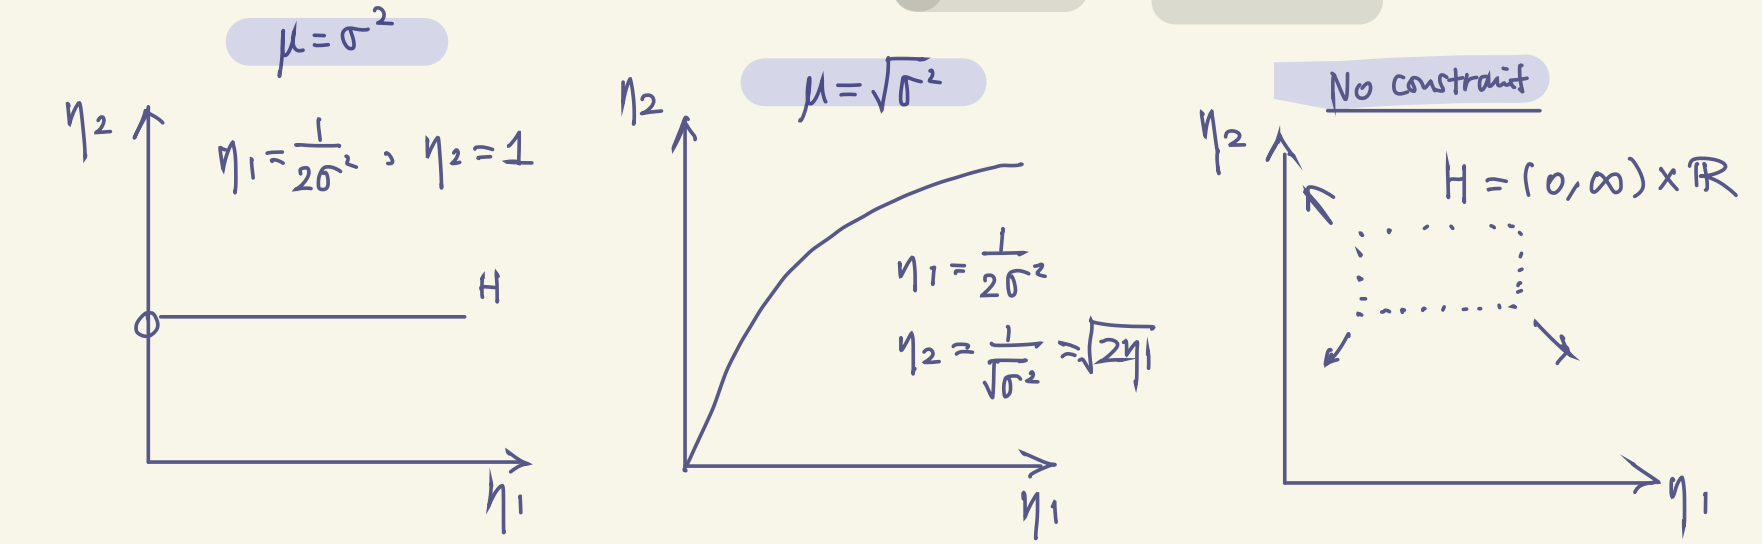
\includegraphics[width=\textwidth]{figures/fullrank-curved.png}
    \caption{curved exponential family}
    \label{fig:fullrank_curved}
\end{figure}

\begin{note}
    \textbf{Properties of Exponential Families}
    \begin{enumerate}[{(1)}]
        \item If $X_1,\cdots,X_n\overset{iid}{\sim}p(x;\theta)=
        \exp\{\sum_{i=1}^s\eta_i(\theta)T_i(x)-B(\theta)\}h(x)$, then,
        by NFFC, 
        \begin{gather}
            T=(\sum_{j=1}^nT_1(X_j),\cdots,\sum_{j=1}^nT_s(X_j))
        \end{gather}
        is sufficient.
        The exponential family data is highly compressible.
        \item If $f$ is integrable, and $\eta\in\Omega$, then
        \begin{gather}
            G(f,\boldsymbol{\eta})=\int{f(x)\exp\{\sum_{i=1}^s\eta_iT_i(x)\}h(x)d\mu(x)}
        \end{gather}
        is infinitely differentiable with respect to $\eta$ and the derivatives
        can be obtained by differentiating it under the integral sign.
        \item Moments of $T_i$'s. Take $f(x)\equiv 1$, then
        {\scriptsize
        \begin{align}
            G(1,\boldsymbol{\eta})
            =&\int{\exp\left\{ \sum_{i=1}^s\eta_iT_i(X) \right\}}h(x)d\mu(x)=\exp\{A(\boldsymbol{\eta})\}\\
            \frac{\partial{G(1,\boldsymbol{\eta})}}{\partial{\eta_i}}
            =& \int{T_i(x)\exp\left\{\sum_{i=1}^s\eta_iT_i(x)\right\}}h(x)d\mu(x)
            =\frac{\partial{A(\boldsymbol{\eta})}}{\partial{\eta_i}}=\exp\{A(\boldsymbol{\eta})\}\\
            \frac{\partial{A(\boldsymbol{\eta})}}{\partial{\eta_i}}
            =& \int{T_i(x)\exp\left\{ \sum_{i=1}^s\eta_iT_i(x)-A(\boldsymbol{\eta}) \right\}}h(x)d\mu(x)
            =\mathbb{E}_{\boldsymbol{\eta}}T_i(X)\\
            \frac{\partial^2{A(\boldsymbol{\eta})}}{\partial{\eta_i}\partial{\eta_j}}
            =& \int{T_i(x)(T_j(x)-\frac{\partial{A(\boldsymbol{\eta})}}{\partial{\eta_j}})
            \exp\left\{ \sum_{l=1}^s\eta_lT_l(x)-A(\boldsymbol{\eta}) \right\}}h(x)d\mu(x)\\
            =& \mathbb{E}_{\boldsymbol{\eta}}(T_i(X)T_j(X))
            -\mathbb{E}_{\boldsymbol{\eta}}T_i(X)
            \mathbb{E}_{\boldsymbol{\eta}}T_j(X)\\
            =& \mathrm{Cov}_{\boldsymbol{\eta}}(T_i(X),T_j(X))
        \end{align}}
    \end{enumerate}
\end{note}

\subsection{Minimal sufficiency}
\begin{definition}[Minimal sufficiency]
    A sufficient statistic $T$ is minimal 
    if for every sufficient statistic $T'$ and 
    for every $x,y\in\mathcal{X}$, 
    $T(x)=T(y)$ when $T'(x)=T'(y)$.
    In other words, $T$ is a function of $T'$,
    i.e. there exists a function $f$ such that $T(x)=f(T'(x))$ for any $x\in\mathcal{X}$.
\end{definition}

\begin{theorem}
    Let $\{p(x;\theta):\theta\in\Omega\}$ be a family of densities with respect to some measure $\mu$
    (Lebesgue measure for continuous distribution $dx$; 
    counting measure for discrete distribution $(x_i-x_{i-1})$). 
    Suppose that there exists a statistic $T$ such that, 
    for every $x,y\in\mathcal{X}$,
    \begin{gather}
        p(x;\theta)=c_{x,y}p(y;\theta)\Rightarrow T(x)=T(y)
    \end{gather}
    for every $\theta\in\Omega$ and some $c_{x,y}\in\mathbb{R}$. 
    Then $T$ is a minimal sufficient statistic.
\end{theorem}
\begin{proof}
    We first prove that $T$ is sufficient and then $T$ is minimal.

    ``$\Rightarrow$'' sufficiency for $T$:

    Start with $T(\mathcal{X})=\{t:t=T(x)~\text{for some}~x\in\mathcal{X}\}=$ range of $T$.
    For each $t\in T(\mathcal{X})$, we consider the preimage $A_t=\{x:T(x)=t\}$.
    Then, for any $y\in\mathcal{X}$, we have $y\in A_{T(y)}$ and $x_{T(y)}\in A_{T(y)}$.
    By the definition of $A_t$, we can see that $T(y)=T(x_{T(y)})$.
    Because of the assumption/condistion imposed in the statement,
    \begin{gather}
        p(y;\theta)=c_{y,x_{T(y)}}p(x_{T(y);\theta})\triangleq h(y)g_\theta(T(y))
    \end{gather}
    which implies that $T$ is sufficient as a result of the NFFC.

    ``$\Leftarrow$'' minimality of $T$:

    Consider another sufficient statistic, say $T'$. 
    By NFFC,
    \begin{gather}
        p(x;\theta)=\Tilde{g}_\theta(T'(x))\Tilde{h}(x)
    \end{gather}
    Take any $x$ and $y$ such that $T'(x)=T'(y)$, then
    \begin{align}
        p(x;\theta)
        =& \Tilde{g}_\theta(T'(x))\Tilde{h}(x)\\
        =& \Tilde{g}_\theta(T'(y))\Tilde{h}(y)\cdot\frac{\Tilde{h}(x)}{\Tilde{h}(y)}\\
        \triangleq& p(y;\theta)c_{x,y}
    \end{align}
    
    Hence, $T(x)=T(y)$ by the assumption of the minimal sufficient statistic theorem.
    So $T'(x)=T'(y)$ implies $T(x)=T(y)$ for any sufficient statistic $T'$ and any $x$ and $y$.
    Hence, $T$ is a minimal sufficient statistic.
\end{proof}

\begin{example}

    Let $X_1,\cdots,X_n\overset{iid}{\sim}\mathcal{N}(\mu,\sigma^2)$ with both $\mu$ and $\sigma^2$ unknown.
    Let $\boldsymbol{x}$ and $\boldsymbol{y}$ be any two sample points, 
    and let $(\Bar{x}_n,s_x^2)$ and $(\Bar{y}_n,s_y^2)$
    be the sample means and variances corresponding to 
    the $\boldsymbol{x}$ and $\boldsymbol{y}$ samples, respectively.

    {\footnotesize
    \begin{gather}
        \frac{p(\boldsymbol{x};\mu,\sigma^2)}{p(\boldsymbol{y};\mu,\sigma^2)}
        = \exp\left\{
        -\frac{1}{2\sigma^2}\left[
        -n(\Bar{x}_n^2-\Bar{y}_n^2)
        +2n\mu(\Bar{x}_n-\Bar{y}_n)
        -(n-1)(s_x^2-s_y^2)
        \right]
        \right\}
    \end{gather}}
    
    The ratio will be constant as a function of $\boldsymbol{\theta}=(\mu,\sigma^2)$
    if and only if $\Bar{x}_n=\Bar{y}_n$ and $s_x^2=s_y^2$. 
    Thus, by the ``theorem'', $(\Bar{x}_x,s_x^2)$ is a minimal sufficient statistic for $\boldsymbol{\theta}$,
    where $s_x^2=\frac{1}{n-1}\sum_{i=1}^n(x_i-\Bar{x}_n)^2$
\end{example}

\begin{example}
    \textbf{Curved exponential family}

    Let $X_1,\cdots,X_n\overset{iid}{\sim}\mathcal{N}(\sigma,\sigma^2)$, where $\sigma>0$, then $\theta=\sigma$
    \begin{gather}
        \frac{p(\boldsymbol{x};\mu,\sigma^2)}{p(\boldsymbol{y};\mu,\sigma^2)}
        = \exp\left\{
        -\frac{1}{2\sigma^2}\left(\sum_{i=1}^n{x_i^2}-\sum_{i=1}^n{y_i^2}\right)
        +\frac{1}{\sigma}\left(\sum_{i=1}^n{x_i}-\sum_{i=1}^n{y_i}\right)
        \right\}
    \end{gather}
    
    This ratio will be constant as a function of $\theta=\sigma$
    if and only if 
    $\sum_{i=1}^n{x_i}=\sum_{i=1}^n{y_i}$ and 
    $\sum_{i=1}^n{x_i^2}=\sum_{i=1}^n{y_i^2}$.
    Thus, by the above theorem, 
    \begin{gather}
        T(\boldsymbol{X})=(\sum_{i=1}^n X_i, \sum_{i=1}^n X_i^2)
    \end{gather}
    is minimal sufficient.
\end{example}

\begin{note}
    If $p(x;\theta)=c_{x,y}p(y;\theta)$ and $x$ and $y$ must be supported by the same $\theta$.
    (Support of $X: \{x\in\mathcal{X}:p(x;\theta)>0\}$).
    Otherwise, the ``constant'' $c_{x,y}$ will be $\theta$-dependent.
\end{note}

\begin{example}
    Let $X_1,\cdots,X_n\overset{iid}{\sim}\text{Uniform}(0,\theta)$ 
    and $T(\boldsymbol{X})=\max_{1\leq i\leq n} X_i \triangleq X_{(n)}$.
    In that case, for $\boldsymbol{x}=(x_1,\cdots,x_n)$ such that $x_i>0$,
    for $i=1,\cdots,n$,
    \begin{gather}
        p(\boldsymbol{x};\theta)
        =\prod_{i=1}^n \frac{1}{\theta}\mathbb{I}(x_i\leq \theta)
        =\frac{1}{\theta^n}\mathbb{I}\left(
        x_{(n)} < \theta
        \right)
    \end{gather}

    If $T(\boldsymbol{x})=T(\boldsymbol{y})$,
    then $p(\boldsymbol{x};\theta)=1\times p(\boldsymbol{y};\theta)$.
    The ratio between the two distributions does not depend on $\theta$,
    so $T$ is sufficient.
    
    Conversely, if $\boldsymbol{x},\boldsymbol{y}>\boldsymbol{0}$ 
    (i.e. $x_i,y_i>0$ for $i=1,\cdots,n$) are supported by the same $\theta$, then
    \begin{gather}
        \{\theta~\text{supporting}~\boldsymbol{x}\}=(T(\boldsymbol{x}),\infty)
        =(T(\boldsymbol{y}),\infty)=\{\theta~\text{supporting}~\boldsymbol{y}\}
    \end{gather}
    Therefore, $T(\boldsymbol{x})=T(\boldsymbol{y})$ and $T$ is a minimal sufficient statistic.
\end{example}

\subsection{Ancillarity \& Completeness}

\begin{example}
    Consider $X_1,\cdots,X_n\overset{iid}{\sim}\text{CauchyLoc}(\theta)$,
    whose distribution is given by 
    \begin{gather}
        p(x;\theta)=\frac{1}{\pi}\cdot\frac{1}{1+(x-\theta)^2}=f(x-\theta)
    \end{gather}
    We can see that $(X_{(1)},\cdots,X_{(n)})$ is minimal sufficient
    \footnote{refer to TPE 1.5}. 
    This is also true for the double exponential location model
    \footnote{jump diffusion;
    refer to Kou, 2002, MS}
    : $p(x,\theta)\propto\exp{(|x-\theta|)}$
\end{example}

\begin{question}
    What determines the level of compressibility?
\end{question}

\begin{definition}[Ancillarity]
    A statistic $A$ is ancillary for $X\sim p_\theta \in \mathcal{P}$
    if the distribution of $A(\boldsymbol{X})$ does not depend on $\theta$.
\end{definition}

\begin{example}
    Consider again $X_1,\cdots,X_n\overset{iid}{\sim}\text{CauchyLoc}(\theta)$,
    and define $A(\boldsymbol{X})=X_{(n)}-X_{(1)}$,
    which can be rewritten as $A(\boldsymbol{X})=(Z_{(n)}+\theta)-(Z_{(1)}+\theta)$,
    and we can see that $A(\boldsymbol{X})$ is ancillary w.r.t. $\theta$
\end{example}

\begin{solution} 
    Answer for Question 1.\\
    The statistic that we make use of should include as little ancillary information as possible.
\end{solution}

\begin{definition}[first-order ancillary statistic]
    A statistics $A$ is first-order ancillary for $X\sim p_\theta\in\mathcal{P}$
    if $\mathbb{E}_\theta A(\boldsymbol{X})$ does not depend on $\theta$.
\end{definition}

\begin{definition}[Completeness]
    A statistic $T$ is complete for $X\sim p_\theta\in\mathcal{P}$
    if no non-constant function of $T$ is first-order ancillary.
    In other words, if $\mathbb{E}_\theta{f(T(\boldsymbol(X)))}=0~\forall{\theta}$,
    thus $f(T(\boldsymbol{X}))=0$ with probability 1 for all $\theta$.
\end{definition}

Completeness formalizes our ideal concept of optimal data reduction.
Minimal sufficiency is our achievable notion of optimal data reduction.

\textbf{Properties}:
\begin{enumerate}
    \item If $T$ is complete sufficient, then $T$ is minimal sufficient. 
    This is known as Bahadur's theorem.
    \item Complete sufficient statistics yield optimal unbiased estimators
\end{enumerate}

\begin{example}
    Let $X_1,\cdots,X_n\overset{iid}{\sim}\text{Bernoulli}(\theta),~\theta\in(0,1)$.
    Then we know that $T(\boldsymbol{X})=\sum_{i=1}^n{X_i}$ is sufficient.
    Sippose $\mathbb{E}_\theta f(T(\boldsymbol{X}))=0$ for all $\theta\in(0,1)$. Observe
    \begin{gather}
        \mathbb{E}_\theta f(T(\boldsymbol{X}))
        =\sum_{i=1}^n{f(i)\binom{n}{i}\theta^i(1-\theta)^{n-i}}=0~\forall{\theta}\in(0,1)\label{eq:compex1}
    \end{gather}
    Dividing Equation (\ref{eq:compex1}) through by $\theta^n$ and let $\beta=\frac{\theta}{1-\theta}$, we have
    \begin{gather}
        \sum_{i=1}^n{f(i)\binom{n}{i}\beta^i}=0~\forall{\beta}>0.\label{eq:compex2}
    \end{gather}

    If $f$ are non-zero, then the LHS of Equation (\ref{eq:compex2}) is a polynomial of degree at most $n$.
    However, an n-th degree polynomial can have at most n roots. 
    Hence, it is impossible for the LHS to equal 0 for every $\beta>0$ unless $f=0$.
    We can conclude that $T$ is complete.
\end{example}

\begin{example}
    Let $X_1,\cdots,X_n\overset{iid}{\sim}\mathcal{N}(\theta,\sigma^2)$, with $\theta\in\mathbb{R}$ unknown and 
    a known $\sigma^2>0$, Is $\Bar{X}_n=\frac{1}{n}\sum_{i=1}^nX_i$ 
    (we know it minimal sufficient) complete for this model?

    To simplify the notation, we consider a special case where $n=1$ and $\sigma=1$,
    so that $T(X)=X\sim \mathcal{N}(\theta,1)$. Suppose
    \begin{gather}
        \mathbb{E}_\theta f(X)
        =\frac{1}{\sqrt{2\pi}}\int_{-\infty}^\infty{f(x)\exp\{-\frac{(x-\theta)^2}{2}\}}dx=0
        ~\forall\theta\in\mathbb{R}.\label{eq:minicompex}
    \end{gather}
    Multiplying both sides by $\sqrt{2\pi}e^\frac{\theta^2}{2}$,
    we can rewrite Equation (\ref{eq:minicompex}) as 
    \begin{gather}
        \int_{\infty}^\infty{f(x)\exp\{ -\frac{x^2}{2}\}\exp\{\theta x\}}dx=0
        ~\forall{\theta}\in\mathbb{R}\label{eq:minicompex2}
    \end{gather}
    
    We decompose $f$ into its positive and negative parts as $f=f^+-f^-$, 
    where $f^+(x)=\max(f(x),0)$ and $f^-(x)=\max(-f(x),0)$.
    Observe that $f^+(x)\geq 0$ and $f^-(x)\geq 0$ for all $x\in\mathbb{R}$ and
    $f^+(x)=f^-(x)$ if and only if $f^+(x)=f^-(x)=0$.
    If $f(x)\geq 0$ a.e. or $f(x)\leq 0$ a.e., 
    then Equation (\ref{eq:minicompex2}) implies that $f(x)=0$ a.e. because
    setting $\theta=0$ gives us an integral of a non-negative (or a non-positive) function.

    We may write
    \begin{gather}
        \frac{\int_{-\infty}^\infty{\color{red}f^+(x)\exp\{-\frac{x^2}{2}\}}\exp\{\theta x\}dx}
        {\color{red}\int_{-\infty}^\infty f^+(x)\exp\{-\frac{x^2}{2}\}dx}
        =
        \frac{\int_{-\infty}^\infty{\color{blue}f^-(x)\exp\{-\frac{x^2}{2}\}}\exp\{\theta x\}dx}
        {\color{blue}\int_{-\infty}^\infty f^-(x)\exp\{-\frac{x^2}{2}\}dx}
        \label{eq:minicompex3}
    \end{gather}
    Notice that in Equation (\ref{eq:minicompex3}), 
    the part of {\color{red} red} or {\color{blue} blue} defines a legitimate probability density and 
    notice that both sides of Equation (\ref{eq:minicompex3}) is the MGF of this density. We have 
    \begin{gather}
        M_{f^+}(t)=M_{f^-}(t)
    \end{gather}
    which implies that $f^+(x)=f^-(x)$ a.e. or, in other words, 
    $f^+=f^-=0$ a.e., i.e. $f(X)=0$ a.s.. 
    Hence $T$ is sufficient and complete.
\end{example}

\begin{exercise}
    If $X\sim p(x;\theta)\propto h(x)\exp\{\theta x\}$, then the statistic $T(X)=X$ is complete.

    \textbf{Keysteps:}
    \begin{enumerate}[{(1)}]
        \item Suppose $\int{f(x)h(x)\exp\{\theta x\}}dx=0~\forall{\theta}$;
        \item Decompose $f=f^+-f^-$ with $f^+,f^-\geq 0$;
        \item $f^+$ and $f^-$ can be viewed as legitimate density;
        \item The decomposition shows that the MGF's of $f^+$ and $f^-$ coincide and hence $f\equiv{0}$.
    \end{enumerate}
\end{exercise}

\begin{theorem}
    $(T_1,\cdots,T_s)$ is complete for any s-dimensional full rank exponential family\footnote{TSH}.
\end{theorem}

\begin{theorem}
    \textbf{Basu's Theorem}\\
    If $T$ is complete and sufficient for $\mathcal{P}=\{p_\theta:\theta\in\Omega\}$
    and $V$ is ancillary, then $T(\boldsymbol{X})\vperp V(\boldsymbol{X})$.
\end{theorem}
\begin{proof}
    Define $q_A(t)=P_\theta(V\in A|T=t)$ and $p_A=P_\theta(V\in A)$.
    By sufficiency and ancillarity, neither $p_A$ nor $q_A(t)$ depends on $\theta$.
    By smoothing/tower expectation, 
    we can write
    \begin{gather}
        p_A=P_\theta(V\in A)=\mathbb{E}_\theta P_\theta(V\in A|T)=\mathbb{E}_\theta q_A(T)
    \end{gather}
    By completeness,
    \begin{gather}
        \mathbb{E}_\theta(q_A(T)-p_A)\triangleq\mathbb{E}_\theta{f(T)}=0
    \end{gather}
    Hence, 
    \begin{gather}
        f(T)=q_A(T)-p_A=0~\text{i.e.}~q_A(T)=p_A
    \end{gather}
    Again by smoothing/tower expectation,
    \begin{align}
        P_\theta(T\in B,V\in A)
        =& \mathbb{E}_\theta[\bm{1}_B(T)\bm{1}_A(V)]~~{\color{gray} \bm{1}_B(T)=\mathbb{I}(T\in B)}\\
        =& \mathbb{E}_\theta\{\mathbb{E}_\theta[\bm{1}_B(T)\bm{1}_A(V)|T]\}\\
        =& \mathbb{E}_\theta\{\bm{1}_B(T)\mathbb{E}_\theta[\bm{1}_A(V)|T]\}\\
        =& \mathbb{E}_\theta[\bm{1}_B(T)q_A(T)]\\
        =& \mathbb{E}_\theta[\bm{1}_B(T)p_A]\\
        =& p_A\mathbb{E}_\theta\bm{1}_B(T)\\
        =& P_\theta(V\in A)P_\theta(T\in B)
    \end{align}
    Hence, $T$ and $V$ are independent as $A$ and $B$ are arbitrary Beorel sets.
\end{proof}

\begin{example}
    Let $X_1,\cdots,X_n\overset{iid}{\sim}\mathcal{N}(\mu,\sigma^2)$, 
    where both $\mu$ and $\sigma^2$ are unknown. 
    Then $\Bar{X}_n\vperp\frac{1}{n}\sum_{i=1}^n(X_i-\Bar{X}_n)^2$.
    
    For any $\sigma>0$, we consider the submodel $\mathcal{P}_\sigma\{\mathcal{N}(\mu,\sigma^2):\mu\in\mathbb{R}\}$.
    In each submodel, $\Bar{X}_n$ is complete and sufficient, 
    and $\frac{1}{n}\sum_{i=1}^n(X_i-\Bar{X}_n)^2$ is ancillary. 
    (Let $X_i=Z_i+\mu$, then $X_i-\Bar{X}_n=Z_i-\Bar{Z}_n$, 
    which does not depend on $\mu$.)

    By Basu's theorem, $\Bar{X}_n\vperp\sum_{i=1}^n(X_i-\Bar{X}_n)^2$
    under $\mathcal{N}(\mu,\sigma^2)$ for any $\mu$.
    Since $\sigma$ is arbitrary, we can conclude that 
    $\Bar{X}_n\vperp\frac{1}{n}\sum_{i=1}^n(X_i-\Bar{X}_n)^2$
    holds for the full model $\mathcal{P}=\{\mathcal{N}(\mu,\sigma^2):\mu\in\mathbb{R},\sigma^2>0\}$.
\end{example}

\subsection{From Data Reduction to Optimal Inference}
\begin{enumerate}
    \item Lossless data reduction (Sufficiency)
    \item Optimal data reduction (Minimal sufficiency + completeness)
    \item \textbf{Optimal inference/estimation}
\end{enumerate}

\begin{definition}[Convex function]
    A function $f$ is a convex function if $x\neq y$ and $\gamma\in(0,1)$
    \begin{gather}
        f(\gamma x+(1-\gamma) y) \leq \gamma f(x) + (1-\gamma) f(y)
    \end{gather}

    The function $f$ is said to be strictly convex if the above inequality holds strictly (i.e. ``$<$'').
\end{definition}


\begin{example}
    As Shown in Figure \ref{fig:convex}
    \begin{enumerate}
        \item For any $\theta\in\Omega$, the function $f(d)=(d-\theta)^2$ is strictly convex on $\mathbb{R}$.
        \item For any $\theta\in\Omega$, the function $f(d)=|d-\theta|$ is convex but not strictly convex.
    \end{enumerate}
\end{example}

\begin{figure}[htpb]
    \centering
    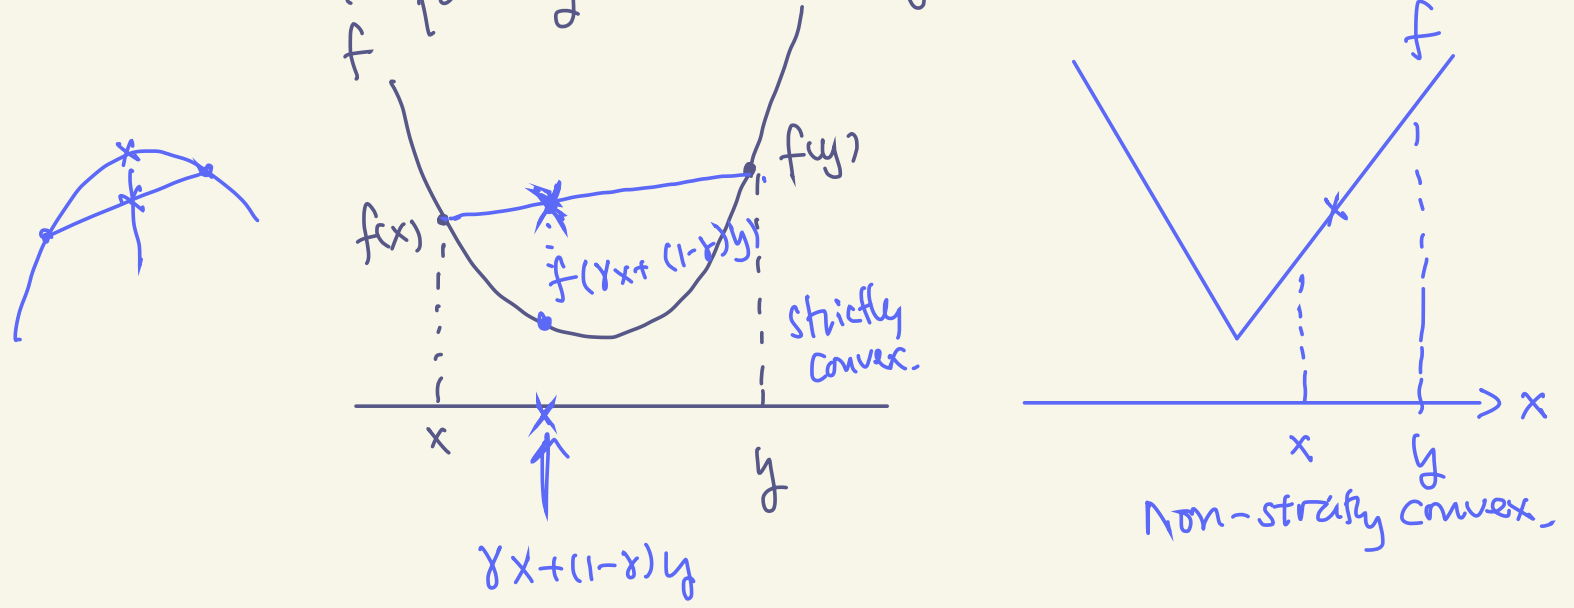
\includegraphics[width=\textwidth]{figures/convex.png}
    \caption{Convex functions}
    \label{fig:convex}
\end{figure}

\begin{theorem}
    \textbf{Jensen's Inequality}\\
    For a convex $f$, and $\mathbb{E}X$ exists, then
    \begin{gather}
        f(\mathbb{E}X)\leq\mathbb{E}f(X)
    \end{gather}
    If $f$ is strictly convex, then the above inequality holds strictly unless 
    $X=\mathbb{E}X$ with probability 1.
\end{theorem}


\begin{theorem}\label{thm:raoblackwell}
    \textbf{Rao-Blackwell Theorem}\\
    Suppose $T$ is sufficient for $\mathcal{P}=\{p_\theta: \theta\in\Omega\}$,
    that $\delta(\boldsymbol{X})$ is an estimator for $g(\theta)$ for which $\mathbb{E}\delta(\boldsymbol{X})$ exists,
    and that $R(\theta,\delta)=\mathbb{E}_\theta L(\theta,\delta(\boldsymbol{X}))<\infty$.
    If, in particular, $L(\theta,\cdot)$ is convex, then
    \begin{gather}
        R(\theta, \eta)\leq R(\theta,\delta)\\
        \text{for}~\eta=\mathbb{E}[\delta(\boldsymbol{X})|T(\boldsymbol{X})]
    \end{gather}
    If $L(\theta,\cdot)$ is strictly convex, then $R(\theta,\eta)<R(\theta,\delta)$
    for any $\theta$ unless $\eta(T(\boldsymbol{X}))=\delta(\boldsymbol{X})$ with probability 1.
\end{theorem}


\begin{example}
    If $X_1,\cdots,X_n\overset{iid}{\sim}\text{Bernoulli}(\theta)$, where $\theta\in(0,1)$.
    Consider $L(\theta,d)=(\theta-d)^2$. 
    Suppose we have a naive estimator $\delta(\boldsymbol{X})=X_1$.
    We know that $T(X)=\Bar{X}_n$ is sufficient,
    so we can apply the Rao-Blackwell Theorem to \textbf{improve an estimator $\delta$}:
    \begin{align}
        \eta(T(\boldsymbol{X}))
        =& \mathbb{E}[\delta(\boldsymbol{X})|T(\boldsymbol{X})]\\
        =& \frac{1}{n}\sum_{i=1}^n\mathbb{E}[\delta(\boldsymbol{X})|\Bar{X}_n]\\
        =& \mathbb{E}(\Bar{X}_n|\Bar{X}_n) = \Bar{X}_n
    \end{align}
    Recall that 
    \begin{gather}
        R(\theta,\eta)=\frac{\theta(1-\theta)}{n}<\theta(1-\theta)=R(\theta,\delta)
    \end{gather}
\end{example}

\newpage